% !TeX root = ../tjuthesis-example.tex

\begin{mdframed}[linewidth=0]
  \begin{longcode}
	\caption{神经网络初值训练,保存和调用}
	\inputminted[numbers=left,
		  frame=single,
		  fontsize=\scriptsize,
		  python3 = true,
		  breaklines=true]
		  {python}{codes/deepritz_2.py}
  \end{longcode}
\end{mdframed}

\matlabinputlisting[caption={主函数}]{codes/test.m}
\matlabinputlisting[caption={Jacobi-Davidson迭代法}]{codes/jacobi_davidson.m}
\matlabinputlisting[caption={两水平区域分解算子}]{codes/twolevel_precondition.m}

%%% Code from Dr. Christian ------ for not using headers.----------------------
\pgfkeysifdefined{/pgfplots/table/output empty row/.@cmd}{
  % upcoming releases offer this more convenient option:
  \pgfplotstableset{
	empty header/.style={
	  every head row/.style={output empty row},
	}
  }
}{
  % versions up to and including 1.5.1 need this:
  \pgfplotstableset{
	empty header/.style={
	  typeset cell/.append code={%
		\ifnum\pgfplotstablerow=-1 %
		  \pgfkeyssetvalue{/pgfplots/table/@cell content}{}%
		\fi
	  }
	}
  }
}
%%%-----------------------------------------------

\pgfplotstabletypeset[
  empty header,
  begin table=\begin{longtable},
  every first row/.append style={before row={%
  \caption{This is a Table with Data}%
  \label{tab:DataTable}\\\toprule
  \textbf{column 1} &\textbf{column 2} \\ \toprule
  \endfirsthead
  %
  \multicolumn{2}{c}%
  {{\bfseries Table \thetable\ Continued from previous page}} \\
  \toprule
  %
  \textbf{column 1} &\textbf{column 2} \\ \toprule
  \endhead
  %
  \midrule \multicolumn{2}{r}{{Continued on next page}} \\ \bottomrule
  \endfoot
  %
  \midrule
  \multicolumn{2}{r}{{Concluded}} \\ \bottomrule
  \endlastfoot
  }},%
  %
  end table=\end{longtable},
  col sep=comma,
  string type,
  ]{tables/data.csv}

\begin{algorithm}[H]
	\caption{两水平加性Schwarz预条件处理的Jacobi-Davidson迭代法}\label{alg:twolevel}
	\begin{algorithmic}
	  \State{给定初值$u^{1}$,终止准则$\varepsilon$,
	  $\lambda^{1} = Rq(u^{1})$, $W^{1} = \mathrm{span}\{u^{1}\}$.设
	  $\lambda^{1}_h \leq \lambda^{1} \leq \lambda^{1}_H$.}
	  \While{$\vert \lambda^{k+1}-\lambda^{k}\vert \geq \varepsilon$}
		\Loop
		\State{
		  计算$t^{k+1}\in \mathrm{span}\{u^{k}\}^{\bot}$
		  \begin{equation}
			(Bt^{k+1},v) = (r^k,v), \quad \forall v \in \mathrm{span}\{u^{k}\}^{\bot}
		  \end{equation}
		  并写为预条件子形式
		  \begin{equation}
			t^{k+1} = (B^{k})^{-1} r^{k} + \beta (B^{k})^{-1} u^{k}
		  \end{equation}
		  其中$\beta$是保证正交的系数.
		}
		\State{
		  将搜索空间扩展为$W^{k+1} = \mathrm{span} \{ W^{k},t^{k+1}\}$.并更新$u^{k+1}$
		  \begin{equation}
			u^{k+1} = \arg\min_{\norm{u^{k+1}}=1} Rq(v),v\in W^{k+1}
		  \end{equation}
		}
		\State{
		  $\lambda^{k+1} \gets Rq(u^{k+1})$
		}
		\EndLoop
	  \EndWhile
	\end{algorithmic}
\end{algorithm}

\begin{figure}
	\begin{center}
	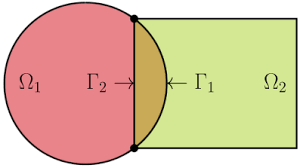
\includegraphics[]{figures/Schwarz_Alternating.png}
	\caption{Schwarz交替法的重叠划分示意图}
	\end{center}
\end{figure}
